%++++++++++++++++++++++++++++++++++++++++
% Don't modify this section unless you know what you're doing!
\documentclass[letterpaper,12pt]{article}
\usepackage{tabularx} % extra features for tabular environment
\usepackage{amsmath}  % improve math presentation
\usepackage{graphicx} % takes care of graphic including machinery
\usepackage[margin=1in,letterpaper]{geometry} % decreases margins
\usepackage{cite} % takes care of citations
\usepackage[final]{hyperref} % adds hyper links inside the generated pdf file
\usepackage{listings}
\usepackage{xcolor}

\definecolor{backcolour}{rgb}{0.95,0.95,0.92}

\lstdefinestyle{mystyle}{
    backgroundcolor=\color{backcolour},
    basicstyle=\ttfamily\footnotesize,    
    breaklines=true,   
    captionpos=b,                    
    keepspaces=true,                 
    numbers=left,                    
    numbersep=5pt,                  
    showspaces=false,                
    showstringspaces=false,
    showtabs=false,                  
    tabsize=2
}

\lstset{style=mystyle}

\hypersetup{
	colorlinks=true,       % false: boxed links; true: colored links
	linkcolor=blue,        % color of internal links
	citecolor=blue,        % color of links to bibliography
	filecolor=magenta,     % color of file links
	urlcolor=blue         
}
%++++++++++++++++++++++++++++++++++++++++


\begin{document}

\title{Bicycle project crowd evaluation}
\author{Hugo Dalboussiere}
\date{\today}
\maketitle

\begin{abstract}
In this experiment we will analyze the accuracy of a crowd of annotators which had to answer the following binary question: ‘‘Do you see a bicycle?’’.
\end{abstract}


\section{Introduction}

Each annotator is given a set of tasks (work package) that it has to solve. Every task is pointing to a specific image hosted on Amazon S3. Based on this image, the annotator should determine if it contains a bicycle or not. After the annotator has handled all its assigned tasks, the results are sent back to the main server and aggregated for later data analysis. The objective of this experiment will be to analyse the results of the annotators which are stored in a JSON file.

\newpage

\section{JSON file format inspection}

It is essential to be comfortable with the format of the given data set in order to exploit them efficiently and accurately. The JSON file weights about 64MB and is not prettified, making it challenging to visualize it in a proper way.
After prettifying the file and stripping off unnecessary data, we have a sample file that is adequate to start taking a look at the different properties of the file (see
figure~\ref{lst:json}).
\renewcommand{\lstlistingname}{Figure}
\renewcommand{\thelstlisting}{2}
\begin{lstlisting}[caption={Content of a prettified sample of the JSON file},captionpos=b,label={lst:json}]
{
  "results": {
    "root_node": {
      "gui_type": "discrete_answer",
      "results": {
        "7e8984b6-dff7-4015-865a-b721a2faf681": {
          "results": [
            {
              "task_input": {
                "image_url": "https://qm-auto-annotator.s3.eu-central-1.amazonaws.com/bicycles/img_4686.jpg"
              },
              "created_at": "2021-02-25T14:08:11.319438+00:00",
              "workpackage_total_size": 5,
              "loss": 0.0,
              "project_node_input_id": "7e8984b6-dff7-4015-865a-b721a2faf681",
              "project_node_output_id": "0000439a-96ac-4bd4-8753-a4baa229ecf2",
              "task_output": {
                "answer": "no",
                "cant_solve": false,
                "corrupt_data": false,
                "duration_ms": 997
              },
              "user": {
                "vendor_id": "vendor_01",
                "id": "08af8775-a72c-4c59-b60f-9ce7df04fa92",
                "vendor_user_id": "annotator_12"
              },
              "root_input": {
                "image_url": "https://qm-auto-annotator.s3.eu-central-1.amazonaws.com/bicycles/img_4686.jpg"
              },
              "project_root_node_input_id": "7e8984b6-dff7-4015-865a-b721a2faf681"
            }
          ],
          "gui_type": "discrete_answer"
        }
      }
    }
  }
}
\end{lstlisting}

The file contains two first higher levels that not bringing much value: ‘‘results’’ and ‘‘root\_node’’. However, the second ‘‘results" property contained in the ‘‘root\_node’’ property is a key element. It contains a set of key and values: the key is the unique identifier of a work package and the value contains an array of results. Each entry in this array is the result of a single task. Each task contains some metadata, such as the annotator id (user id), crowd (vendor), task duration and the image url, but most importantly it contains the answer returned by the annotator: ‘‘yes’’ or ‘‘no’’.

\section{Data Preparation}

A JSON file can be manipulated using Python thanks to the ‘‘json’’ library, but it is easier to manipulate data models rather than dictionaries as they have no predefined structure. Data models\footnote{See ‘‘Data model’’ from the Python documentation: https://docs.python.org/3/reference/datamodel.html} can be assimilated to classes in Object Oriented Programming (OOP) and have many advantages (re-usability, maintainability, code readability...). For this use case, one of the most interesting benefits of data models is having a loose coupling to the format of the JSON file: if the data format of the file were to change, the only adaptation needed would be how the data models are created, but the business logic leveraging these data models would remain unchanged.
Two data models will be created: Annotator and Task (see
figure~\ref{fig:data_models})

\renewcommand\thefigure{3}
\begin{figure}[hb] 
        \centering 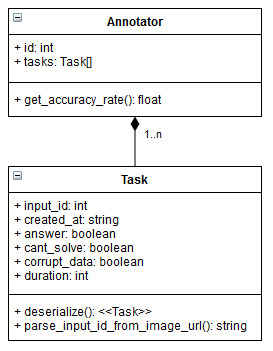
\includegraphics{uml.PNG}
        \caption{
                \label{fig:data_models}
                UML diagram of the data models
        }
\end{figure}

\newpage
\section{Analysis}
The data set contains 22 annotators. The minimum annotation time is -99999ms, while the maximum annotation time is 42398ms. These numbers alone do not give much insight on the whole data set, and having a negative time is most likely the outcome of an error during the aggregation of the results. The histogram in figure~\ref{fig:question_1_b} allows us to have an overview of the distribution of the duration time.

\renewcommand\thefigure{4}
\begin{figure}[hb] 
        \centering 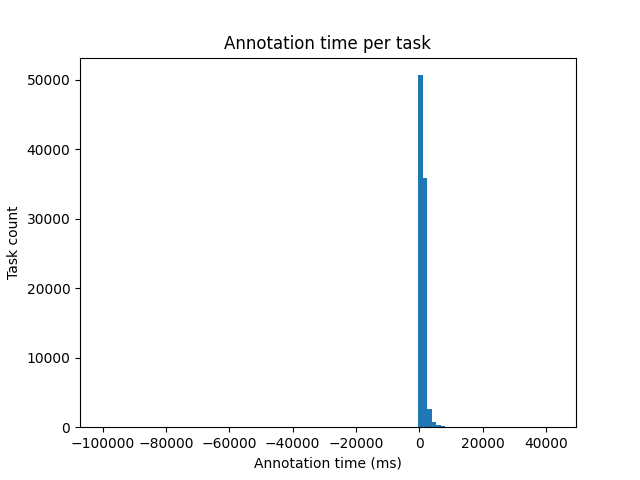
\includegraphics{question_1_b.PNG}
        \caption{
                \label{fig:question_1_b}
                Annotation time per task
        }
\end{figure}

While it is clear that most of the tasks take between 0 and 5000ms to execute, the histogram is hard to read because of the very few outlier values in the data set. In the next histogram (see figure~\ref{fig:question_1_b_no_outliers}), outlier values ($<$ 0ms or $>$ 5000ms) are excluded.

\newpage
\renewcommand\thefigure{5}
\begin{figure}[hb] 
        \centering 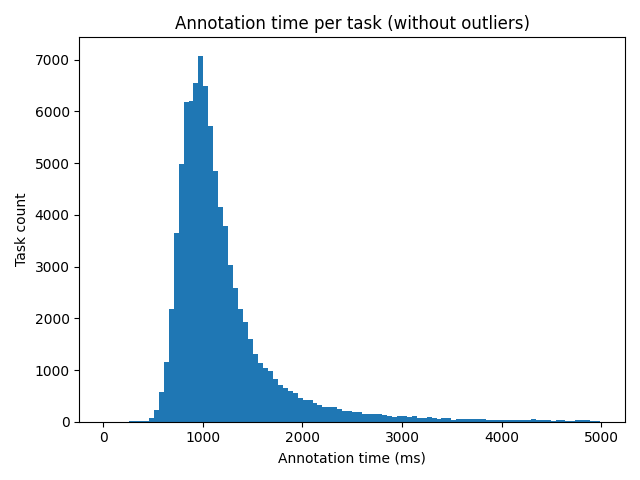
\includegraphics{question_1_b_no_outliers.PNG}
        \caption{
                \label{fig:question_1_b_no_outliers}
                Annotation time per task (without outliers)
        }
\end{figure}

It's now clear that most of the tasks take between 500 and 1500ms to complete. The average annotation time is 1284ms, but it is more accurate to use the median time as we have outlier values. The median average annotation time is 1058ms.

\newpage
Annotators each produced between 170 to 7596 results (see figure~\ref{fig:question_1_c}). A result corresponds to an annotated task.

\renewcommand\thefigure{6}
\begin{figure}[hb] 
        \centering 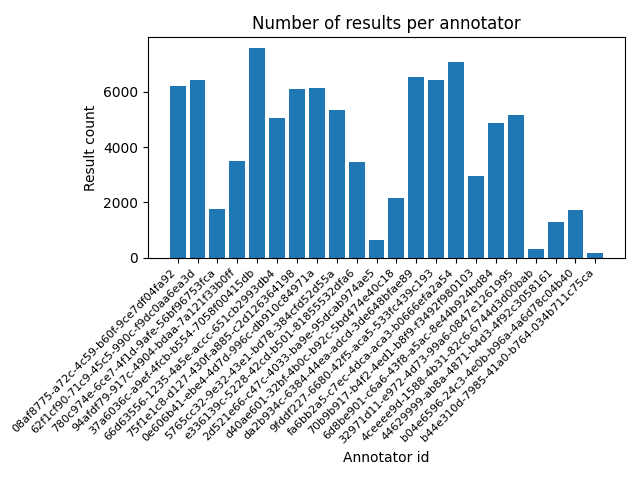
\includegraphics{question_1_c.PNG}
        \caption{
                \label{fig:question_1_c}
                Number of results per annotator
        }
\end{figure}

\newpage
Out of 9087 distinct inputs, 384 of them have a high variance (v $>$ 0.2), meaning annotators highly disagree on approximately 4.2\% of questions. The table in figure~\ref{fig:question_1_4} shows the 10 questions with the highest answer variance, sorted in descending order.

\renewcommand\thefigure{7}
\begin{figure}[hb] 
\centering
        \begin{tabular}{|ccc|} 
\hline
\multicolumn{1}{|c}{input id} & \multicolumn{1}{c}{V} & \multicolumn{1}{c|}{Answers} \\
\hline
2207 & 0.25 & 0, 0, 1, 1, 1, 1, 0, 1, 0, 0 \\
5914 & 0.25 & 1, 0, 1, 1, 0, 0, 1, 0, 0, 1 \\
0998 & 0.25 & 0, 0, 1, 0, 1, 1, 1, 0, 0, 1 \\
2940 & 0.25 & 1, 0, 1, 1, 1, 0, 0, 0, 1, 0 \\
8397 & 0.25 & 1, 0, 0, 0, 1, 0, 1, 1, 1, 0 \\
3654 & 0.25 & 0, 1, 1, 1, 0, 0, 1, 1, 0, 0 \\
5958 & 0.25 & 0, 0, 0, 1, 1, 0, 1, 0, 1, 1 \\
0627 & 0.25 & 0, 1, 1, 1, 1, 0, 0, 0, 0, 1 \\
0669 & 0.25 & 0, 0, 0, 1, 0, 1, 1, 0, 1, 1 \\
6324 & 0.25 & 0, 1, 0, 0, 0, 1, 1, 1, 0, 1 \\
\hline
\end{tabular}
        \caption{
                \label{fig:question_1_4}
                Questions with the highest variance with their answers
        }
\end{figure}

When treating each task, annotators had the chance to indicate if the data was corrupted, or if they could not solve the task.
Out of 90870 tasks, 17 of them could not be solved and 4 of them had corrupt data.
All of these tasks answered ‘‘no’’ to the question and had an average annotation time well below average: 838ms for tasks that could not be solved and 461ms for tasks with corrupt data.
It is interesting to note that among the 22 annotators present in this experiment, only 10 of them contributed to the 17 tasks mentioned above.
\newline
\newline
The reference set is balanced, with 49.5\% of thruthy values and 50.5\% of falsy values (see figure~\ref{fig:question_3}).

\renewcommand\thefigure{8}
\begin{figure}[hb] 
        \centering 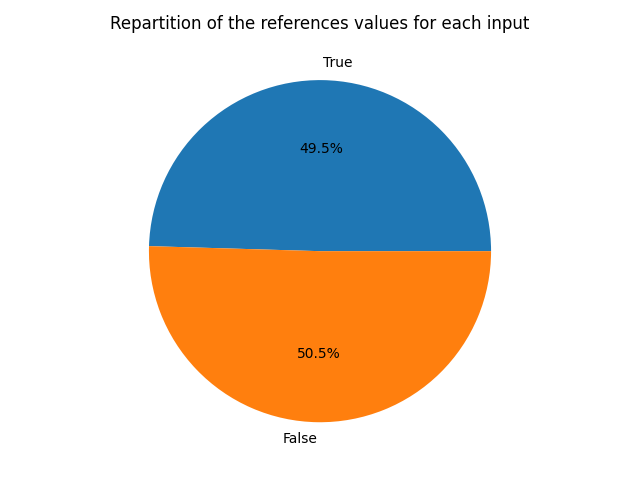
\includegraphics[scale=0.63]{question_3.PNG}
        \caption{
                \label{fig:question_3}
                Repartition of the references values for each input
        }
\end{figure}

Using the reference set, we can compare the output of each annotator to the expected answers, and compute an accuracy rate. The vast majority of annotators (90.9\%) have an accuracy rate higher than 90\% (see figure~\ref{fig:question_4}).
With an average annotator accuracy rate of 93.5\%, the overall performance is good but it would be interesting to identify the best and worst performing annotators.

\renewcommand\thefigure{9}
\begin{figure}[hb] 
        \centering 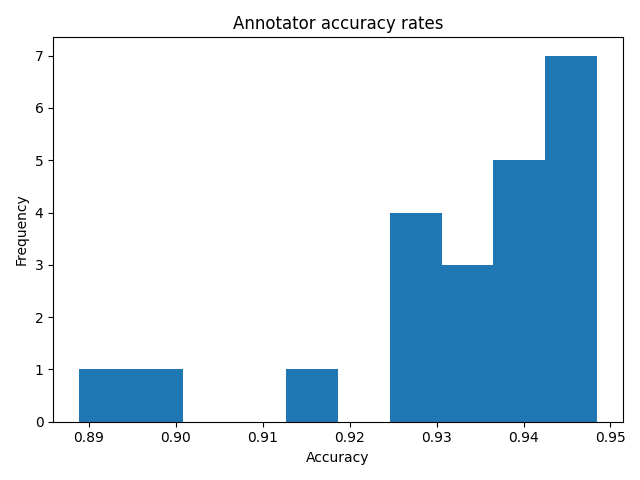
\includegraphics[scale=0.7]{question_4.PNG}
        \caption{
                \label{fig:question_4}
                Annotator accuracy rates
        }
\end{figure}

Based on the computed accuracy rate of each annotator and their average task duration, we can easily rank them to retrieve the ten worst performing annotators (see figure~\ref{fig:question_4_b}).

\renewcommand\thefigure{10}
\begin{figure}[hb] 
\centering
        \begin{tabular}{|ccc|} 
\hline
\multicolumn{1}{|c}{Annotator id} & \multicolumn{1}{c}{Accuracy rate (\%)} & \multicolumn{1}{c|}{Average task duration (ms)} \\
\hline
4ceeee9d-1588-4b31-82c6-6744d3d00bab & 88.89 & 1253 \\
da2b934c-6384-44ea-adcd-3de648bfae89 & 89.93 & 1435 \\
d40ae601-32bf-4b0c-b92c-5bd474e40c18 & 91.54 & 1578 \\
5765cc32-9e32-43e1-bd78-384cfd52d55a & 92.66 & 1497 \\
9fddf227-6680-42f5-aca5-533fc439c193 & 92.84 & 1114 \\
2d521e66-c47c-4033-ba9e-95dcab974ae5 & 92.86 & 1460 \\
08af8775-a72c-4c59-b60f-9ce7df04fa92 & 92.98 & 1306 \\
6d8be901-c6a6-43f8-a5ac-8e44b924bd84 & 93.33 & 1199 \\
37a6036c-a9ef-4fcb-b554-7058f00415db & 93.48 & 1178 \\
62f1cf90-71c9-45c5-990c-f9dc0aa6ea3d & 93.65 & 1280 \\
\hline
\end{tabular}
        \caption{
                \label{fig:question_4_b}
                Worst performing annotators
        }
\end{figure}

\newpage
Similarly, we can retrieve the ten best performing annotators (see figure~\ref{fig:question_4_c}).

\renewcommand\thefigure{11}
\begin{figure}[hb] 
\centering
        \begin{tabular}{|ccc|} 
\hline
\multicolumn{1}{|c}{Annotator id} & \multicolumn{1}{c}{Accuracy rate (\%)} & \multicolumn{1}{c|}{Average task duration (ms)} \\
\hline
75f1e1c8-d127-430f-a885-c2d126364198 & 94.84 & 1365 \\
44629999-ab8a-4871-b4d3-4f92c3058161 & 94.84 & 1077 \\
0e606b41-ebe4-4d7d-996c-db910c84971a & 94.83 & 1173 \\
b44e310d-7985-41a0-b764-034b711c75ca & 94.71 & -1303 \\
fa6bb2a5-c7ec-4dca-aca3-b0666efa2a54 & 94.69 & 1155 \\
b04e6596-24c3-4e0b-b96a-4a6d78c04b40 & 94.67 & 1595 \\
780c974e-6ce7-4f1d-9afe-56bf96753fca & 94.33 & 879 \\
66d63556-1235-4a5e-accc-651cb2993db4 & 94.23 & 1270 \\
94afdf79-917c-4904-bdaa-7a121f33b0ff & 94.2 & 992 \\
70b9b917-b4f2-4ed1-b8f9-f3492f980103 & 94.0 & 1239 \\
\hline
\end{tabular}
        \caption{
                \label{fig:question_4_c}
                Best performing annotators
        }
\end{figure}

In the two previous figures, the ranks are solely based on the accuracy rate. Ideally, other criteria should also be taken into account: difficulty of the task (depending on the average annotator percentage of correctness), task duration.\newline
We can imagine a ranking system where each annotator is awarded a number of points on completion of a task. Task results with a wrong answer will not be rewarded. The number of points rewarded for each task will be computed based on the following equation:
\begin{equation}
\nonumber
task\_points = 10 (\frac{avg\_task\_duration\_time}{task\_duration\_time}) (1 + (1 - task\_completion\_percentage^{\mathrm{2}}))
\end{equation}

Using this ranking system, the best performing annotators are the one with the highest average points per task (see figure~\ref{fig:question_4_d}).

\renewcommand\thefigure{12}
\begin{figure}[hb] 
\centering
        \begin{tabular}{|ccc|} 
\hline
\multicolumn{1}{|c}{Annotator id} & \multicolumn{1}{c}{Average points per task}  & \multicolumn{1}{c|}{Rank difference with figure 11} \\
\hline
780c974e-6ce7-4f1d-9afe-56bf96753fca & 30.87 & $\uparrow$ 6 \\
94afdf79-917c-4904-bdaa-7a121f33b0ff & 25.65 & $\uparrow$ 7 \\
44629999-ab8a-4871-b4d3-4f92c3058161 & 24.55 & $\downarrow$ 1 \\
9fddf227-6680-42f5-aca5-533fc439c193 & 23.61 & $\uparrow$ 14 \\
62f1cf90-71c9-45c5-990c-f9dc0aa6ea3d & 23.46 & $\uparrow$ 8 \\
fa6bb2a5-c7ec-4dca-aca3-b0666efa2a54 & 23.11 & $\downarrow$ 1 \\
4ceeee9d-1588-4b31-82c6-6744d3d00bab & 23.07 & $\uparrow$ 15 \\
0e606b41-ebe4-4d7d-996c-db910c84971a & 22.55 & $\downarrow$ 5 \\
70b9b917-b4f2-4ed1-b8f9-f3492f980103 & 22.44 & $\uparrow$ 1 \\
37a6036c-a9ef-4fcb-b554-7058f00415db & 22.29 & $\uparrow$ 4 \\
\hline
\end{tabular}
        \caption{
                \label{fig:question_4_d}
                Best performing annotators based on computed score
        }
\end{figure}

\newpage
In order to better visualize if there is any correlation between annotators accuracy rate and the average task duration, a scatter plot would be ideal. As seen in figure~\ref{fig:question_4_e}, there doesn't seem to be any correlation between the two criterias.

\renewcommand\thefigure{13}
\begin{figure}[hb] 
        \centering 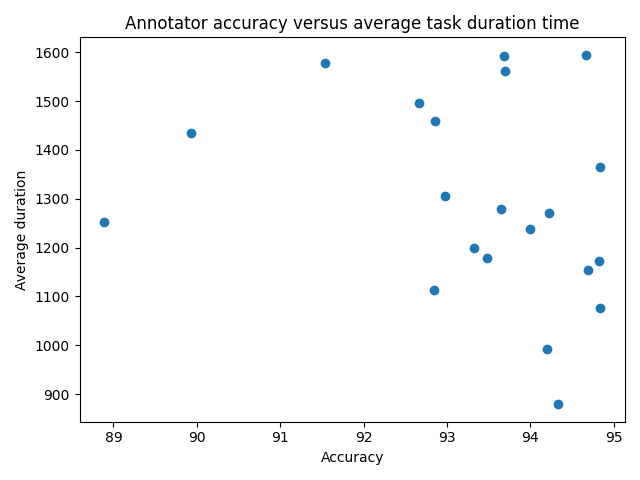
\includegraphics{question_4_e.PNG}
        \caption{
                \label{fig:question_4_e}
                Annotator accuracy rates
        }
\end{figure}

\newpage
\section{Conclusions}
This experiment allowed us to learn about interesting key performance indicators such as the average processing time of a task, or the performance of annotators based on the reference data.\\
The moderate size of the JSON file containing the results facilitated the processing and analysis of the data, but the current approach could be problematic with a higher number of results: from a certain threshold, it would no longer be possible to load the complete data set in memory.\\
To overcome this problem, different options are possible: batch processing, use of a database which is optimized to handle large volumes of data, .
The extracted data of the data set being relational, it would be ideal to insert them in a relational database (type Postgresql) in order to be able to execute SQL queries. SQL queries are very fast and flexible and are used across different systems (Postgresql, MySQL, Oracle, Amazon Athena...).\\
Moreover, the migration to a database would be very easy by using the existing models in the Python code and an ORM. ORMs allow querying and manipulating data in a relational database using an object-oriented paradigm.

\end{document}
